\documentclass[11pt,a4paper]{report}
\usepackage[cp1250]{inputenc}
\usepackage[english]{babel}
\usepackage[IL2]{fontenc}
\usepackage{amsmath}
\usepackage{amsfonts}
\usepackage{amssymb}
\usepackage{makeidx}
\usepackage{graphicx}
\usepackage{lmodern}
\usepackage{subfig}
\usepackage[autostyle]{csquotes}
\usepackage{setspace}
\usepackage[
backend=bibtex        % if we want unicode
,style=iso-authoryear % or iso-numeric for numeric citation method
,autolang=other       % to support multiple languages in bibliography      
]{biblatex}

\usepackage{titlesec}    
\titleformat{\chapter}[block]
{\normalfont\Large\bfseries}{\thechapter.}{1em}{\Large}
\titlespacing*{\chapter}{0pt}{-19pt}{19pt}


\titleformat{\section}[block]
{\normalfont\large\bfseries}{\thesection.}{1em}{\large}
\titlespacing*{\section}{0pt}{11pt}{19pt}


\usepackage{scrpage2}
\ifoot[]{}
\cfoot[]{}
\ofoot[\pagemark]{\pagemark}


\newcommand{\fakeparagraph}[1]{%
	\par\refstepcounter{paragraph}% Increase paragraph counter
	\paragraphmark{#1}% Add paragraph mark (header)
}



\graphicspath{ {./images/} }

\makeatletter
\def\blx@maxline{77}
\makeatother

\bibliography{Thesis.bib}

\newcommand*{\captionsource}[2]{%
	\caption[{#1}]{%
		#1%
		\\\hspace{\linewidth}%
		\textbf{Source:} #2%
	}%
}

\pagenumbering{gobble}

\usepackage[left=3.5cm,right=2cm,top=2cm,bottom=2cm]{geometry}
\author{Bc. Michal Koh�tek}
\title{Recognizing the user's emotional state using intelligent control systems}
\begin{document}
	
\begin{titlepage}
	
{\centering
{\bfseries\LARGE UNIVERZITA KON�TANT�NA FILOZOFA V NITRE \par}
{\bfseries\LARGE FAKULTA PR�RODN�CH VIED \par}
\vfill
{\bfseries\LARGE RECOGNIZING THE USER'S EMOTIONAL STATE USING INTELLIGENT 
CONTROL SYSTEMS\par}
\vspace{1cm}
{\bfseries\Large Diploma thesis\par}
\par}
\vfill
\Large{
Study programme:\par
Field of Study:\par
Department:\par
Supervisor: Mgr. Martin Magdin, PhD\par}
\vfill
\textbf{Nitra 2018}\hfill\textbf{Bc. Michal Koh�tek}
\end{titlepage}
\onehalfspacing
\chapter*{Abstract}
\cfoot{}
Abstract goes here

\chapter*{Dedication}
To mum and dad

\chapter*{Declaration}
I declare that..

\chapter*{Acknowledgements}
I want to thank...

\tableofcontents
 
\chapter*{Introduction}
\pagenumbering{arabic}
\setcounter{page}{8}
\pagestyle{scrplain}
\begin{flushright}

"Smiles are probably the most underrated \\ facial expressions, 
 much more complicated \\ than most people realize. 
 There are dozens\\ of smiles, each differing in appearance \\
 and in the message expressed."\\
 - Paul Ekman
\end{flushright}

\paragraph{} Emotions are at the core of the human experience, albeit very hard 
to define, recognize and name, even in yourself. They are, by definition 
different from person to person, in diverse cultures and upbringings. Our 
perception of emotions and their classification has evolved in recent years. 
Various authors has tried to divide our emotional states into basic categories 
such as Ekman's Anger, Fear, Disgust, Happiness, Sadness and Surprise. However, 
recent work by psychologists and historians alike show, that a more complex 
look at emotions might be needed. 

\paragraph{}Emotional recognition changes with time. In 12th century, bards 
looked at yawning not as a sign of boredom or tiredness, but as a sign of a 
hidden and deep love. Early Christians recognized an emotion called "accidie", 
a lethargy and despair brought about by flying demons. Boredom, as such was 
first really  felt by the Victorians as a response to the new ideas of leisure 
time and self-improvement. Among the psychologist, there is a standing question 
whether some cultures feel some hard to define emotions more strongly, because 
they bothered to name them as separate kinds. For example the Russian "toska", 
a longing with nothing to long for, as coined by Vladimir Nabokov. Recent 
developments of cognitive science tell us, that emotions are not just simple 
reflexes, but inherently complex and elastic systems of response towards both 
the biologies 
that we've inherited and the cultures, that we live in now. They are not just 
simple chemistry, but a cognitive phenomena, not shaped only by our body 
functions, but also our thought process, concepts and language. The 
neuroscientist Lisa Feldman Barrett studies this 
dynamic relationship between words and emotions. She argues, that when a person 
learns a new word for an emotion, they also learn to feel and recognize it 
(\cite{barrett}). 
There is a historicity to emotions, they have changed in history, often times 
very dramatically, in response to new cultural expectations, religious beliefs, 
new ideas about gender, age, ethnicity, economical and political ideologies. 

\paragraph{}There is a push to increase our emotional intelligence. Emotions 
are so 
powerful, that in past, they were sometimes thought to be a cause of illness. 
In 17th century, there was a student attending the Swiss university in Basel. 
He 
came afflicted with fever, heart palpitations, skin sores on his body and was 
close to dying. When they sent him back home to die, he started getting better 
and by the time, he returned to his hometown, he almost entirely recovered. In 
1688, Johannes Hoffer, medical doctor, learnt of this case and 
many like it and coined the term for a severe homesickness as "nostalgia". Last 
confirmed death by nostalgia was an American soldier fighting during the First 
World War in France. In early 20th century, this feeling has morphed more into 
a longing for lost time, instead of homesickness and downgraded in severity. 
Nowadays, our culture celebrates happiness, as it is said to make 
us a better workers, parents and partners. However, in 16th century, this 
position was filled by sadness, as is evident by self-help books from that 
period, which tried to encourage sadness in readers by giving them lists of 
reasons to be disappointed.

\paragraph{}In order to study both basic emotions and their mixtures in the 
complex variety, we need appropriate detection and classification tools and 
techniques. Over the years, many psychologists and computer scientist 
collaborated to create a set of markers and techniques recognizing them. We 
will discuss several of them and compare their usefulness, reliability and 
practicality. These methods most often try to detect basic emotions such as the 
seven basic emotions (\cite{Ekman}) or a 12-point Affect Circumplex model 
(\cite{Russel}).
\begin{figure} [ht]
	\centering
	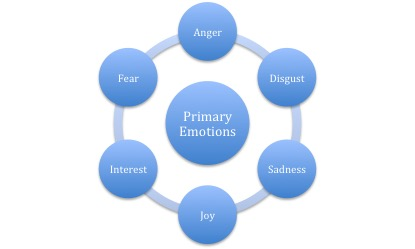
\includegraphics{images/Primary_Emotions}
	\caption{Six primary emotions}
	\label{fig:}
\end{figure} 




\chapter{Emotion classification} \paragraph{}Emotion classification is a 
contested issue in 
emotion research and in affective science. The two fundamental viewpoints of 
affective scientists' approach are: \begin{enumerate}
	\item Emotions as discrete and fundamentally different constructs
	\item Emotions as fluid and characterized on a dimensional basis in 
	groupings
\end{enumerate}
Various categorizations of emotions also vary in description how emotions 
relate to each other.
\section{Discrete models of emotions}
\paragraph{}Discrete emotion theory claims that there is a small 
number 
of core affects. 
This number can vary depending on the proponent, for example Silvan Tomkins 
considered nine basic emotions. Six, that came evolutionarily earlier, 
interest-excitement, enjoyment-joy, surprise-startle, distress-anguish, 
anger-rage, fear-terror, once that evolved later, shame-humiliation and finally 
disgust and dissmell, which he later took back. In the paired affects, the 
first of the pair is the mild manifestation and the second the more intense. 
(\cite{tomkins1962affect}), (\cite{tomkins1963affect}). This model is somewhat 
controversial nowadays among affective theorists, especially over Tomkins' firm 
insistence that there were nine and only nine, biologically based affects. He 
also argued, that these affects are quite discreet (in contrast to the more 
muddled and complex emotions) and that they shared a common biological heritage 
with what Darwin called emotions in animals (\cite{darwin1998expression}). They 
also differ from Freudian drives in lacking an object.
\paragraph{}Similarly, Carroll Izard delineated 12 discrete emotions: 
interest, joy, surprise, sadness, anger, disgust, contempt, self-hostility, 
fear, shame, shyness and guild. He measured these via his Differential Emotion 
Scale (\cite{Izard}). Among other contributors to this theory, such as John 
Watson, Edwin Newman and Ross Buck, Paul Ekman performed a series of 
cross-cultural studies with Carrol Izard and reported that there are at least 
six emotions, that people across the world produce and are able to recognize. 
This was further evidenced when researchers approached the people of New Guinea 
with no previous exposure to Westerners nor their culture. When they showed 
them pictures of people expressing six core emotions, subjects could in fact 
point out the different emotions and distinguish between them 
(\cite{ekmanguinea}). 

\section{Dimensional models of emotions}
\paragraph{} There are various theoretical and practical reasons for which some 
researchers define emotions according to one or more dimensions. Dimensional 
models are an attempt to conceptualize human emotions by defining where they 
lie in two or three dimensions. Most incorporate valence and arousal or 
intensity dimensions. In contrast to theories of basic emotion, which propose 
that different emotions arise from separate neural systems, dimensional models 
suggest that a common and interconnected neurophysiological system is 
responsible for all affective states. (\cite{posner}) 
\paragraph{}In 1897, Wilhelm Max Wundt proposed, that emotions can be described 
by three dimensions: 
"pleasurable versus unpleasurable", "arousing versus subduing" and "strain 
versus relaxation" (\cite{wundt2017outlines}). Later, Harold Schlosberg named 
three dimension, "pleasantness�unpleasantness", "attention�rejection" and 
"level of activation" (\cite{schlosberg1954three}).
\paragraph{}Another model, called the circumplex model, was developed by James 
Russell. This model suggest that emotions are distributed in a two-dimensional 
circular space, containing both arousal and valence dimensions. The vertical 
axis represents arousal, horizontal axis valence and the center of the circle 
represents a neutral valence and medium level of arousal.(\cite{circumplex}).

\begin{figure} [ht]
	\centering
	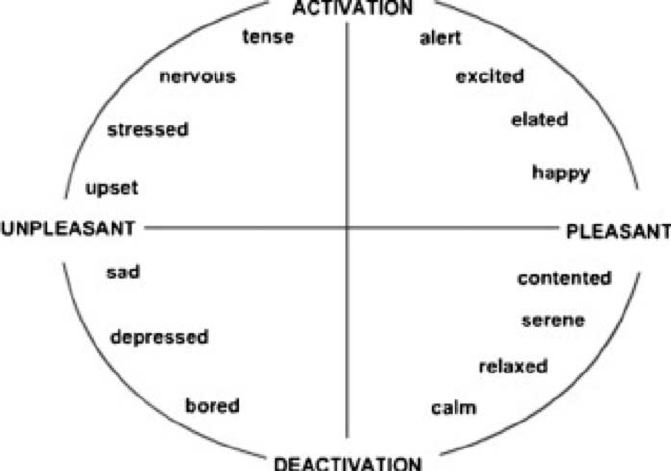
\includegraphics[scale=0.4]{images/russel_model}
	\centering
	\caption{ A. Russell�s (1980) circumplex model of affect}
	\label{fig:}
\end{figure} 

This model was later modified by Russel and Lisa Feldman Barret, which they 
described as representative of core affect, which are the most elementary 
feelings that need not be directed toward anything. Different prototypical 
emotional episodes, or clear emotions that are evoked or directed by specific 
objects, can be plotted on the circumplex, according to their levels of arousal 
and pleasure (\cite{Russell1999CoreAP}).

\paragraph{}Another model of emotion appeared in 1992. This two-dimensional 
model consists of vectors, that point in two directions. The vector model 
assumes that there is always an underlying arousal dimension and that valence 
determines the direction in which a particular emotion lies.
\begin{figure}
		\centering
		\subfloat[label1]{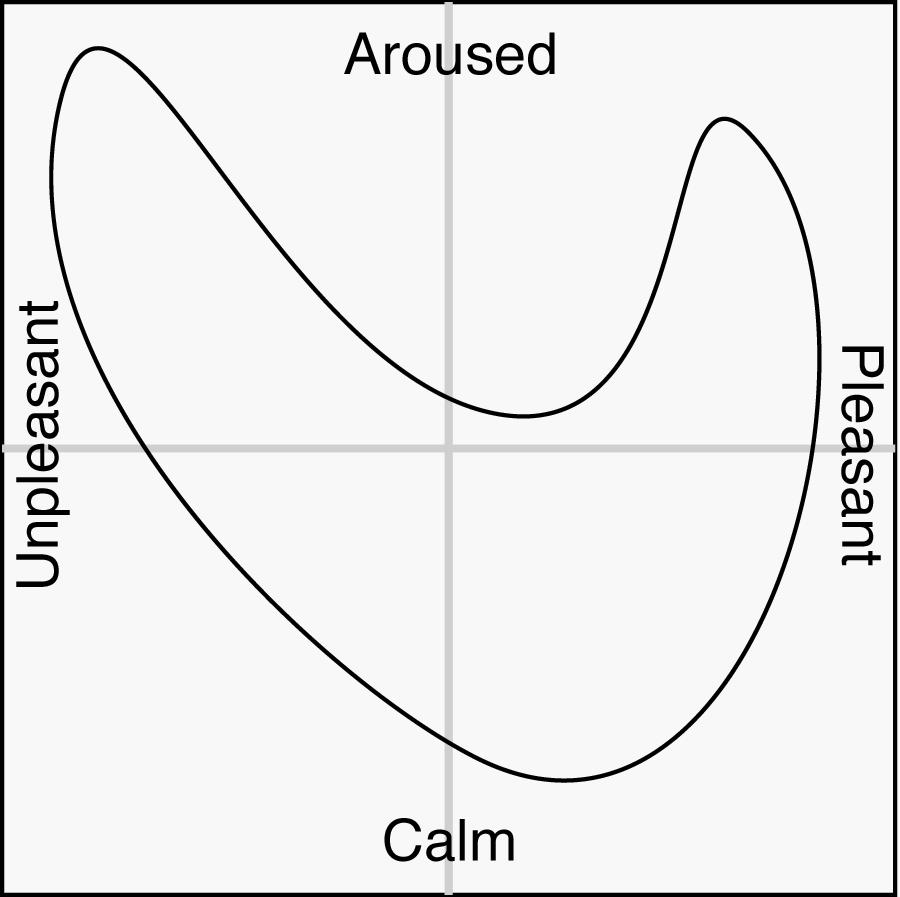
\includegraphics[width=0.2\linewidth]{images/vector0}}%
		\qquad
		\subfloat[label1]{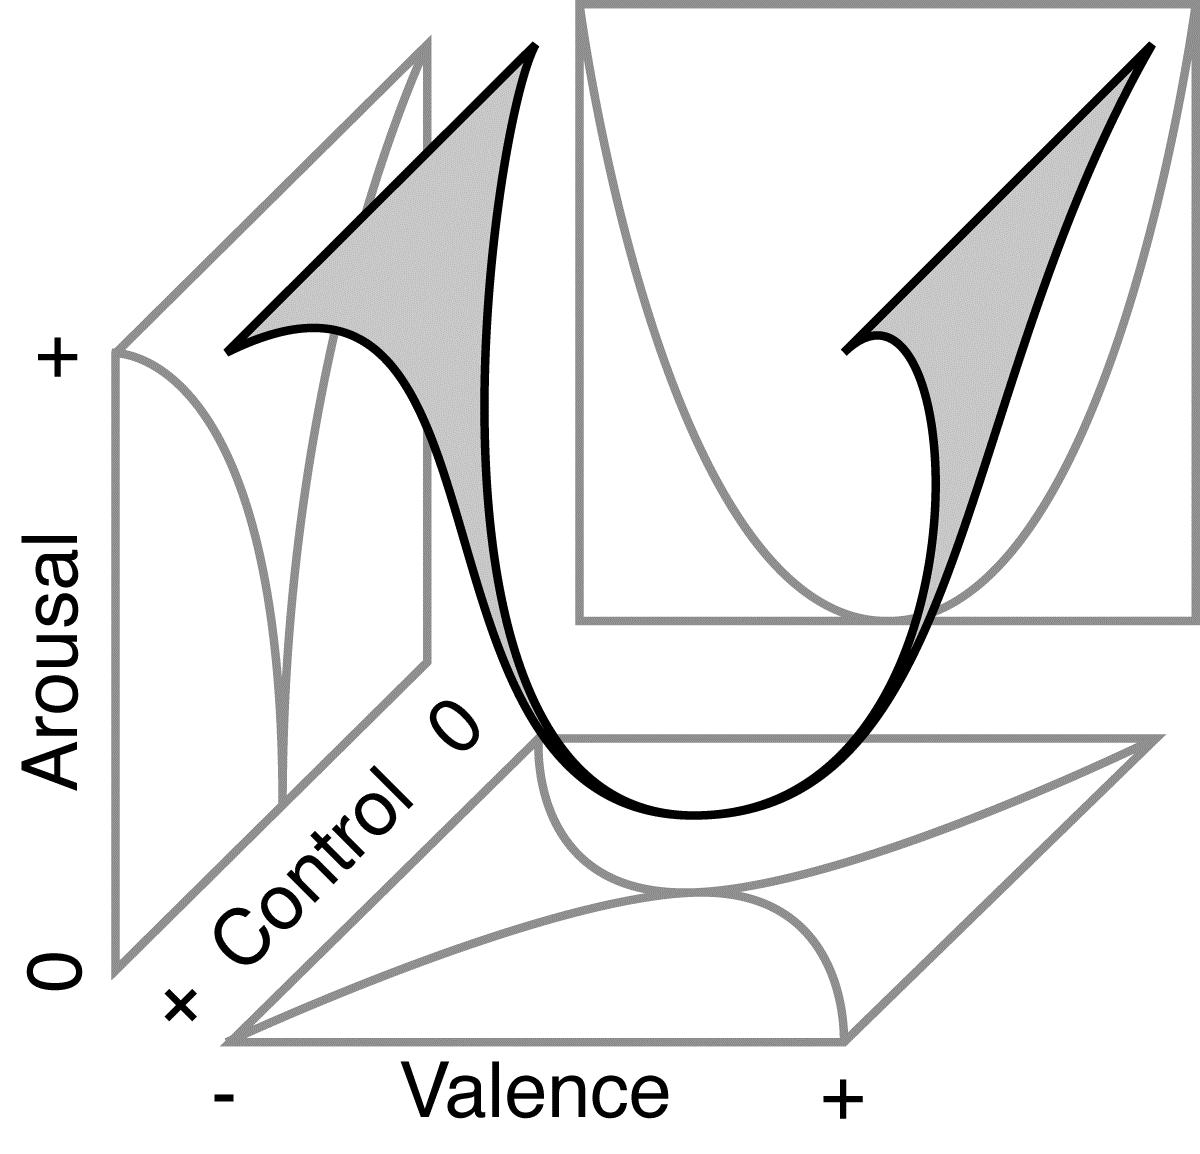
\includegraphics[width=0.2\linewidth]{images/vector1}}%
		\caption{Vector model of emotions}
		\label{fig:}
\end{figure}

\paragraph{} The positive activation � negative activation (PANA) was 
originally created in 1985 by David Watson and Auke Tellegen. It suggests that 
positive and negative affect are two separate systems. Like in the vector 
model, states of higher arousal tend to be defined by their valence and states 
of lower arousal tend to be more neutral in term of valence. In the PANA model, 
the vertical axis represents low to high positive affect and the horizontal 
axis represents low to high negative affect. The dimensions of valence and 
arousal lay at a 45-degree rotation over these axes (\cite{watson}).

\begin{figure} [ht]
	\centering
	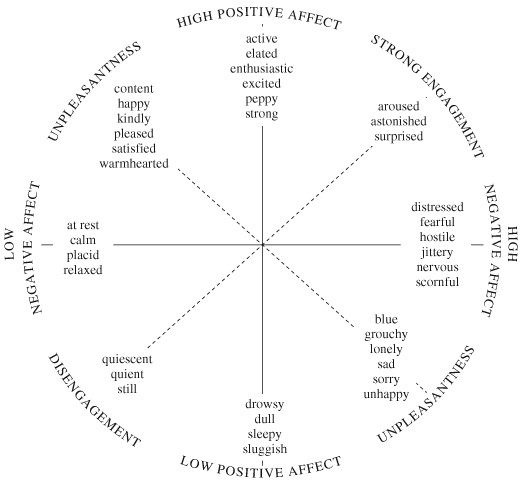
\includegraphics[scale=0.4]{images/consensual}
	\centering
	\caption{Consensual (PANA) model of emotion}
	\label{fig:}
\end{figure}

\paragraph{} In 1980, Robert Plutchik constructed a wheel of emotions. This 
model is a hybrid of both basic-complex categories and dimensional theories. 
Emotions are arranged in concentric circles, with the more basic emotions on 
the inner circles, while the outer circles are occupied by complex emotions.  
Notably, outer circles are also formed by blending the inner circle emotions. 
Plutchik suggested 8 primary contrasting pairs of emotions. Joy/sadness, 
anger/fear, trust/disgust and surprise/anticipation. Like colors, primary 
emotions can be expressed at different intensities and can mix with one another 
to form different emotions (\cite{Plutchik1988}).

\begin{figure} [ht]
	\centering
	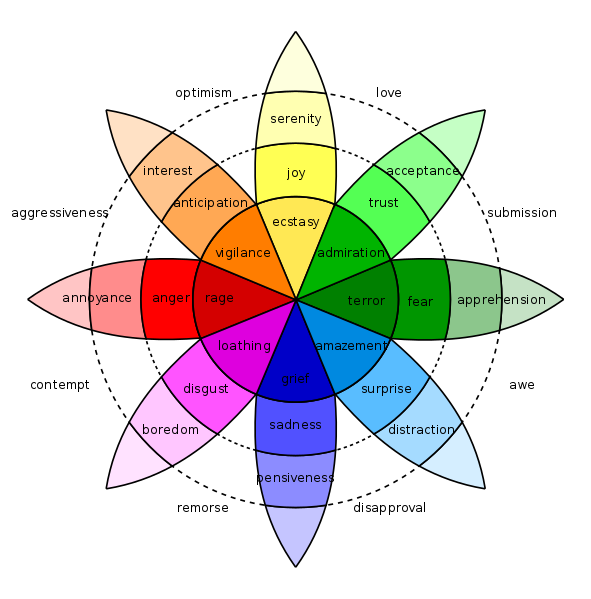
\includegraphics[scale=0.3]{images/Plutchik_wheel}
	\centering
	\caption{Plutchik's wheel of emotions}
	\label{fig:}
\end{figure}

\paragraph{} The PAD emotional state model was developed by Albert Mehrabian 
and James A. Russel. It uses three numerical dimensions, \textbf{P}leasure, 
\textbf{A}rousal, and \textbf{D}ominance to represent all emotions 
(\cite{mehrabian1980basic}). Initially it's use was in a theory of 
environmental psychology, the core idea being that physical environments 
influence people through their emotional impact (\cite{mehrabian1974approach}). 
Subsequently it was used by Peter Lang to propose a physiological theory of 
emotion (\cite{lang}). Furthermore, it was also used by Russel to develop a 
theory of emotional episodes (\cite{coreaffect}). The Pleasure-Displeasure 
Scale measures how pleasant an emotion may be. Anger and fear are, for 
instance, unpleasant emotions and thus score high on the displeasure. 
Contrarily, joy is a pleasant emotion. The Arousal-Nonarousal Scale measures 
the intensity of emotion. For instance while both anger and rage are unpleasant 
emotions, rage is much more intense than anger. Boredom, while also an 
unpleasant state, has a low arousal volume. Lastly, the 
Dominance-Submissiveness Scale shows the dominant nature of the emotion. While 
both fear and anger are unpleasant emotions, anger is dominant, but fear is a 
submissive emotion (\cite{mehrabian1980basic}).
\begin{figure} [ht]
	\centering
	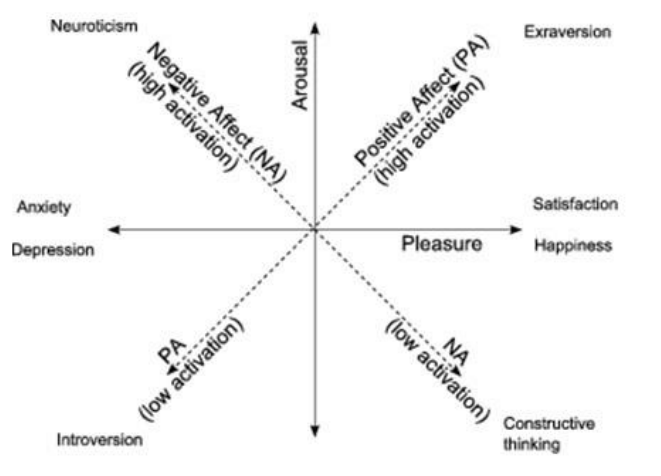
\includegraphics[scale=0.4]{images/pad_model}
	\centering
	\caption{PAD emotional state model}
	\label{fig:}
\end{figure}
A more abbreviated version of the PAD model has also been used in 
organizational studies where the emotions towards specific entities or products 
are measured. It uses just 4 values for each dimension, providing only 64 
values for emotions (\cite{abbrpad}). 

\paragraph{} An example of three-dimensional models, the L�vheim cube of 
emotion was presented where the signal substances (dopamine, noradrenaline and 
serotonin) form the axes of a coordinate system, and the eight basic emotions 
according to Tomkins are placed in the eight corners.
\begin{figure} [ht]
	\centering
	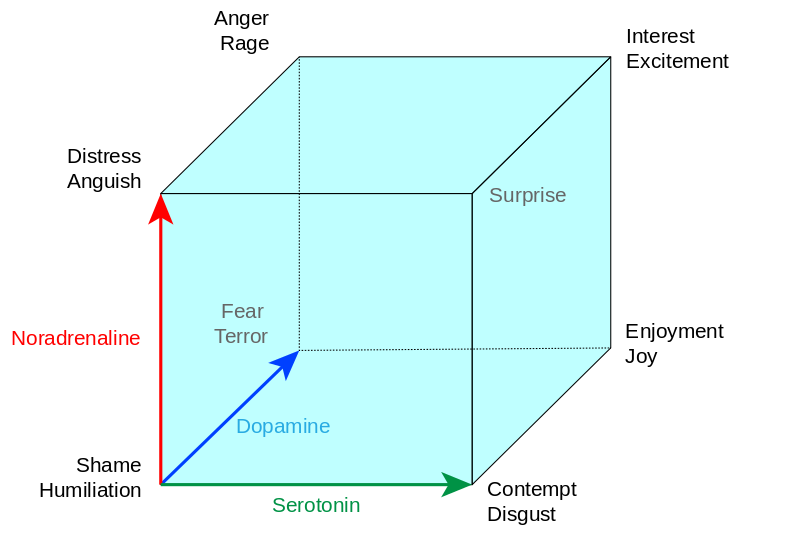
\includegraphics[scale=0.4]{images/lovheimcube}
	\centering
	\caption{L�vheim cube of emotion}
	\label{fig:}
\end{figure}
As shown on the figure below, anger is produced by the combination of low 
serotonin, high dopamine and high noradrenaline. Conversely joy is a product of 
high serotonin, high dopamine and low noradrenaline. Since none of the axis is 
identical to valence \footnote{pleasantness}, the cube seems somewhat rotated 
when 
compared to other models (\cite{Lvheim2012ANT}).


\paragraph{} Most recently Cowen and Kelter, researchers from University of 
California, Berkeley introduced a statistically derived taxonomy of emotion. 
(\cite{Cowen201702247}) \blockquote{Across self-report methods, we find that 
the [2185] 
videos [selected and shown to volunteer subjects] reliably elicit 27 distinct 
varieties of reported emotional experience. Further analyses revealed that 
categorical labels such as amusement better capture reports of subjective 
experience than commonly measured affective dimensions (e.g., valence and 
arousal). Although reported emotional experiences are represented within a 
semantic space best captured by categorical labels, the boundaries between 
categories of emotion are fuzzy rather than discrete. By analyzing the 
distribution of reported emotional states we uncover gradients of emotion�from 
anxiety to fear to horror to disgust, calmness to aesthetic appreciation to 
awe, and others�that correspond to smooth variation in affective dimensions 
such as valence and dominance. Reported emotional states occupy a complex, 
high-dimensional categorical space} 

\paragraph{}More dimensional models of emotion have been developed, though 
there are just a few that remain as the dominant models currently accepted by 
most (\cite{comparison}). There have been observed great cultural differences 
in the way in which emotions are valued, expressed and regulated. The social 
norms for emotions, like the frequency with or circumstances in which they are 
expressed also vary drastically in diverse cultures. An important piece of 
evidence that disputes the universality of emotions is language. Emotions such 
as the schadenfreude \footnote{The experience of pleasure, joy, or 
self-satisfaction that comes from learning of or witnessing the troubles, 
failures, or humiliation of another.} in German and saudade\footnote{Deep 
emotional state of nostalgic or profound melancholic longing for an absent 
something or someone that one loves.} in Portuguese are commonly expressed in 
emotions in their respective languages, but lack an English equivalent. Thus it 
is reasonable in our research to scale back on the complex, culturally 
influenced emotions and focus on the more primal, basic emotions, that may be 
more quantifiable by studying the physiological markers and responses in 
subjects.
\section{Physiological responses of emotions}


\section{Progress in techniques used in research of emotions}
\paragraph{}As we've described motion recognition is an important object of 
studies in today's 
psychology, with many potential uses and applications. Correctly assessing and 
recognizing subject's emotion can lead to better understanding it's motivation 
and inner working. Data gained through methods described below can be used to 
assess the effectiveness of marketing, comprehensibility of lectures, usability 
of user interfaces, measure of impact of psychological therapy, etc. Previous 
implementations of emotion recognition technology often have had a multitude of 
disadvantages, which prohibited it's daily and widespread usage. Therefore, we 
have set upon creating a solution, that is modular, reasonable to wear for 
prolonged durations of time and still maintains a degree of reliability in 
captured data. We can do so by using an array of data resources, that 
complement each other, diminishing their disadvantages and reinforcing 
confidence.
\chapter{Hardware sensors}
\chapter{Software technologies}

\printbibliography
\end{document}